\documentclass[12pt, letterpaper]{article}

\usepackage{amsmath}
\usepackage{pgfplots, pgfplotstable}

\makeatletter
\long\def\ifnodedefined#1#2#3{%
    \@ifundefined{pgf@sh@ns@#1}{#3}{#2}%
}

\pgfplotsset{
    discontinuous/.style={
    scatter,
    scatter/@pre marker code/.code={
        \ifnodedefined{marker}{
            \pgfpointdiff{\pgfpointanchor{marker}{center}}%
             {\pgfpoint{0}{0}}%
             \ifdim\pgf@y>0pt
                \tikzset{options/.style={mark=*}}
                \draw [densely dashed] (marker-|0,0) -- (0,0);
                \draw plot [mark=*, mark options={fill=white}] coordinates {(marker-|0,0)};
             \else
                \tikzset{options/.style={mark=none}}
             \fi
        }{
            \tikzset{options/.style={mark=none}}        
        }
        \coordinate (marker) at (0,0);
        \begin{scope}[options]
    },
    scatter/@post marker code/.code={\end{scope}}
    }
}
\makeatother

\title{Homework 4}
\author{Martin Mueller}
\date{Due: March $1^{st}$, 2019}

\begin{document}
\maketitle

\begin{center}
	\underline{\textbf{Chapter 2}}
\end{center}

\textbf{14. A survey of 1000 people in a city indicates that 34\% have invested in stocks, 48\% have invested in bonds, and 21\% have invested in stocks and bonds.}

\qquad \textbf{a) What is the probability that a randomly selected person from this city has invested in bonds, given that the person has invested in stocks?}

\begin{center}
	Let's define event $A$ to be that the person has invested in stocks and event $B$ to be that the person has invested in bonds:
\end{center}
\begin{align*}
	P(B|A) &= \frac{P(A \cap B)}{P(A)} \\
	&= \frac{P(\text{invested in stocks \textit{and} bonds})}{P(\text{invested in stocks})} \\
	&= \frac{21\%}{34\%} = \boxed{0.6176}
\end{align*}

\pagebreak

\qquad \textbf{b) What is the probability that a randomly selected person from this city has invested in stocks, given that the person has invested in bonds?}

\begin{center}
	This problem is essentially the same as above, except that we are given event $B$ instead of $A$:
\end{center}
\begin{align*}
	P(A|B) &= \frac{P(A \cap B)}{P(B)} \\
	&= \frac{P(\text{invested in stocks \textit{and} bonds})}{P(\text{invested in bonds})} \\
	&= \frac{21\%}{48\%} = \boxed{0.4375}
\end{align*}

\qquad \textbf{c) Are the events "invested in stocks" and "invested in bonds" independent?}

\begin{center}
	One way of telling if two events $A$ and $B$ are independent is by using the following formula: $P(A|B) = P(A)$. $P(A|B)$ was figured out in part b), and $P(A)$ was given in the directions: $P(A|B) = 0.4375$ and $P(A) = 34\% \text{ or } 0.34$. Since $0.4375 \neq 0.34$, events $A$ and $B$ are not independent.
\end{center}

\textbf{17. A single card is drawn from a standard 52 card deck.  If $A$ is the event "the drawn card is black" and $B$ is the event "the drawn card is a multiple of 3"...}

\qquad \textbf{a) ...find $P(B|A)$.}

\begin{center}
	In this case, events $A$ and $B$ are independent (justification given below). Thus, we know that $P(B|A) = P(B)$:
\end{center}
\begin{align*}
	P(B) &= \frac{\text{number of cards that are multiples of 3}}{\text{number of cards in the deck}} \\
	&= \frac{12}{52} \leftarrow \text{(the 3s, 6s, and 9s of each of the 4 suits)}\\
	&= \boxed{0.2308}
\end{align*}

\pagebreak

\qquad \textbf{b) ...are the events $A$ and $B$ independent? Why?}

\begin{center}
	Events $A$ and $B$ are independent because as it states in the directions: "a \textit{single} card is drawn from a standard 52 card deck". This means that the cards are not drawn consecutively, and therefore, each event has no bearing on the other.
\end{center}

\begin{center}
	\underline{\textbf{Chapter 3}}
\end{center}

\textbf{1. A fair die is tossed twice. Let the random variable $X = |\text{first toss outcome} - \text{second toss outcome}|$.}

\qquad \textbf{a) Find the pmf of $X$.}

\begin{center}
	Here's how I visualized it:
	\break
	\break
	\begin{tabular}{c|c|c}
		First toss & Second toss & $|\text{First toss}-\text{Second toss}|$ \\
		\hline
		1 & 1, 2, 3, 4, 5, 6 & 0, 1, 2, 3, 4, 5 \\
		2 & 1, 2, 3, 4, 5, 6 & 1, 0, 1, 2, 3, 4 \\
		3 & 1, 2, 3, 4, 5, 6 & 2, 1, 0, 1, 2, 3 \\
		4 & 1, 2, 3, 4, 5, 6 & 3, 2, 1, 0, 1, 2 \\
		5 & 1, 2, 3, 4, 5, 6 & 4, 3, 2, 1, 0, 1 \\
		6 & 1, 2, 3, 4, 5, 6 & 5, 4, 3, 2, 1, 0
	\end{tabular}
	\break
	\break
	After that, it was pretty easy to count up the values and write out the pmf:
\end{center}
\[
	P(X = x)=
	\left\{
		\begin{tabular}{cc}
			$\frac{6}{36}$ & x = 0 \\[0.07cm]
			$\frac{10}{36}$ & x = 1 \\[0.07cm]
			$\frac{8}{36}$ & x = 2 \\[0.07cm]
			$\frac{6}{36}$ & x = 3 \\[0.07cm]
			$\frac{4}{36}$ & x = 4 \\[0.07cm]
			$\frac{2}{36}$ & x = 5
		\end{tabular}
	\right.
\]

\pagebreak

\qquad \textbf{b) Find the cdf of $X$ and graph it.}

\begin{center}
	All I have to do is do some addition with the pmf listed above and add corresponding intervals to get the cdf:
\end{center}
\[
	F(x)=
	\left\{
		\begin{tabular}{cc}
			$\frac{0}{36}$ & x $<$ 0 \\[0.07cm]
			$\frac{6}{36}$ & 0 $\le$ x $<$ 1 \\[0.07cm]
			$\frac{16}{36}$ & 1 $\le$ x $<$ 2 \\[0.07cm]
			$\frac{24}{36}$ & 2 $\le$ x $<$ 3 \\[0.07cm]
			$\frac{30}{36}$ & 3 $\le$ x $<$ 4 \\[0.07cm]
			$\frac{34}{36}$ & 4 $\le$ x $<$ 5 \\[0.07cm]
			$\frac{36}{36}$ & x $\ge$ 5
		\end{tabular}
	\right.
\]
{\centering
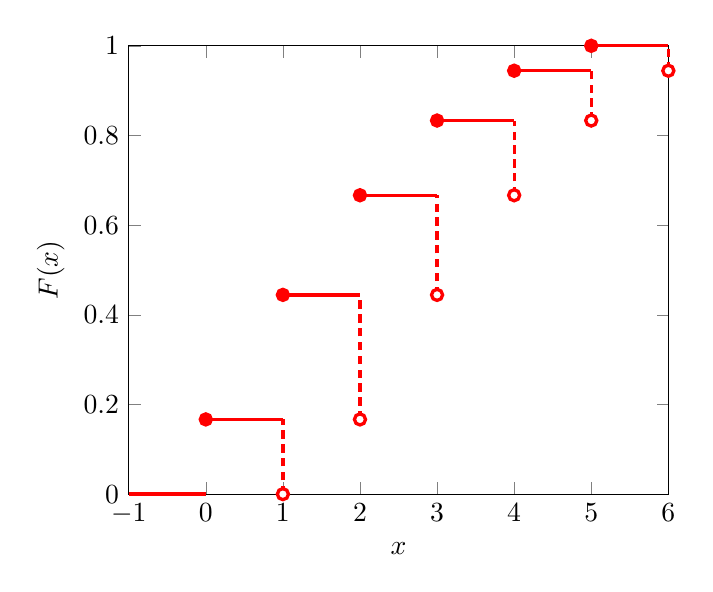
\begin{tikzpicture}
\begin{axis}[
	xlabel=$x$,
	ylabel=$F(x)$,
    clip=false,
    jump mark left,
    ymin=0,ymax=1,
    xmin=-1, xmax=6,
    every axis plot/.style={very thick},
    discontinuous,
    table/create on use/cumulative distribution/.style={
        create col/expr={\pgfmathaccuma + \thisrow{f(x)}}   
    }
]
\addplot [red] table [y=cumulative distribution]{
x f(x)
-1 0
0 6/36
1 10/36
2 8/36
3 6/36
4 4/36
5 2/36
6 0
};
\end{axis}
\end{tikzpicture}
\par}

\pagebreak

\textbf{3. The phone lines to a doctor's office are occupied 20\% of the time. Assume that the event \{lines are occupied on successive calls to the office\} are independent. Four calls are placed to the office. The random variable $X$ denotes  the number of times the lines were not occupied. Find the probability distribution function of $X$.}

\begin{center}
	There are 5 different cases to consider here: the case that $X$ is 0, 1, 2, 3, or 4. Let's take a look at each one individually. If $X=0$, then the phones were not busy each time a call was placed. Since the probability of the phones being busy is $20\%$, the probability of the phones not being busy is the compliment of that: $100\% - 20\% = 80\%$. Now if all of those calls were taken right away, we have $(0.8)^{4}$ which is $0.4096$. For $X=1$, 3 of 4 the calls were taken right away, but 1 of the 4 was not. Since we don't know exactly which one, we have to consider the possibility of each of the 4 calls being the missed one: $(0.8)^{3}{_{4}C_{1}}(0.2)^{1}$ which is $0.4096$. A similar situation applies to the next 2 scenarios: $(0.8)^{2}{_{4}C_{2}}(0.2)^{2} = 0.1536$ and $(0.8)^{1}{_{4}C_{3}}(0.2)^{3} = 0.0256$. As for the last scenario, it is the reverse of the first; instead of all of the calls being taken immediately, all of the phones were initially busy for each of the 4 calls placed: $(0.2)^{4} = 0.0016$. Now if we take these figures and put them into a properly formatted probability distribution function, it should look something like this:
\end{center}
\[
	P(X = x)=
	\left\{
		\begin{tabular}{cc}
			$0.4096$ & x = 0 \\
			$0.4096$ & x = 1 \\
			$0.1536$ & x = 2 \\
			$0.0256$ & x = 3 \\
			$0.0016$ & x = 4 \\
		\end{tabular}
	\right.
\]

\pagebreak

\textbf{5. An insurance company offers its policyholders a number of different premium payment options. For a randomly selected policyholder, let $X$ = the number of months between successive payments. The cdf of $X$ is as follows:}

\[
	F(x)=
	\left\{
		\begin{tabular}{cc}
			0 & x $<$ 1 \\
			.30 & 1 $\le$ x $<$ 3 \\
			.40 & 3 $\le$ x $<$ 4 \\
			.45 & 4 $\le$ x $<$ 6 \\
			.60 & 6 $\le$ x $<$ 12 \\
			1 & x $\ge$ 12
		\end{tabular}
	\right.
\]

\textbf{a) What is the pmf of $X$?}

\begin{center}
	To start, I'm going to make the assumption that the insurance company gives the consumer the option of paying for their coverage on a monthly, quarterly, triannual, biannual, or annual basis. In the context of the problem and considering the values in the cdf, it makes sense. Next, I'll do some simple arithmetic to find the corresponding probability values for each $x$ by taking the difference between a given probability value whose interval starts at the $x$ in question and the preceding probability value. For example: for $X=1$, I'll look at the probability of the interval that starts at $1$ and subtract the preceding probability: $0.30 - 0 = 0.30$. Now I'll do this for each $x$: for $X=3$, $0.40 - 0.30 = 0.10$, for $X=4$, $0.45 - 0.40 = 0.05$, for $X=6$, $0.60 - 0.45 = 0.15$, and finally, for $X=12$, $1 - 0.60 = 0.40$. Now if we take these figures and put them into a properly formatted probability mass function, it should look something like this:
\end{center}
\[
	P(X = x)=
	\left\{
		\begin{tabular}{cc}
			$0.30$ & x = 1 \\
			$0.10$ & x = 3 \\
			$0.05$ & x = 4 \\
			$0.15$ & x = 6 \\
			$0.40$ & x = 12 \\
		\end{tabular}
	\right.
\]

\pagebreak

\textbf{b) Using just the cdf, compute $P(2 < X < 10)$, $P(3 \le X \le 8)$ and $P(4 \le X)$.}

\begin{center}
	For the first probability, since we are dealing with discrete functions, $P(2 < X < 10)$ can be translated into $P(3 \le X \le 9)$, for the next probability, its form doesn't need any altering, and for the last one, it can be rewritten as $1 - P(X \le 3)$. The reason for this is that $P(X \le 3)$ is already listed in the cdf. Now to perform the arithmetic and solve:
\end{center}
\begin{align*}
	P(3 \le X \le 9) = 0.60 - 0.40 = \boxed{0.20} \\
	P(3 \le X \le 8) = 0.60 - 0.40 = \boxed{0.20} \\
	1 - P(X \le 3) = 1 - 0.40 = \boxed{0.60}
\end{align*}
\end{document}